\documentclass[11pt, notheorems]{beamer}
\usepackage[utf8]{inputenc}
\usepackage[croatian]{babel}
\usepackage[T1]{fontenc}
\usepackage{amsmath}
\usepackage{amsfonts}
\usepackage{amssymb}
\usepackage{graphicx}
\usepackage{fixmath}
%\usecolortheme[snowy]{owl}
\usetheme{metropolis}

\newtheorem{theorem}{Teorem}

\newcommand{\q}{\left}
\newcommand{\w}{\right}

\newcommand{\matr}[1]{\mathbold{#1}}
\newcommand{\prob}[1]{\operatorname{\mathbf{P} \q(#1\w)}}

\begin{document}
  \author{Lovre Mrčela}
  \title{Analiza vremenskih nizova zasnovana na kompleksnim mrežama}
  \subtitle{Diplomski rad}
  \institute{Sveučilište u Zagrebu \\
             Fakultet elektrotehnike i računarstva \\
             \textbf{Zavod za elektroničke sustave i obradbu informacija}}
  \date{\today}
  \setbeamertemplate{navigation symbols}{}

  \begin{frame}[plain]
  \maketitle
  \end{frame}

  \begin{frame}{Sadržaj}
    \setbeamertemplate{section in toc}[sections numbered]
    \tableofcontents[hideallsubsections]
  \end{frame}
  
  \section{Uvod}
  \begin{frame}
    \frametitle{Cilj rada}
    \begin{itemize}
    \item optimizacija portfelja
    \item unaprjeđenje postojećih metoda \alert{statističke arbitraže}
    \item modeliranje \emph{interakcija vrijednosnica} korištenjem \alert{kompleksnih mreža}
    \end{itemize}
  \end{frame}

  \begin{frame}
    \frametitle{Teorem o nearbitraži}
    \begin{theorem}
      Ako je u trenutku 0 vrijednost portfelja $V\q(0\w) = 0$, tada je u nearbitražnim okolnostima vjerojatnost $\prob{V\q(t\w) > 0} = 0$ za $t > 0$.
    \end{theorem}
  \end{frame}

  \begin{frame}
    \frametitle{Koeficijent obrtaja}
    \begin{itemize}
      \item \emph{mjera promjenljivosti} portfelja
      \item u rasponu $\q[0, 2\w]$
      \item portfelj s $N$ vrijednosnica $\matr{\alpha} = \begin{bmatrix} \alpha_1 & \alpha_2 & \cdots & \alpha_N \end{bmatrix}$
      \item \alert{koeficijent obrtaja} $\eta^{(t)}$:
      \begin{equation*}
        \eta^{(t)} = \sum_{i=1}^{N} \q \lvert \alpha_i^{(t)} - \alpha_i^{(t-1)} \w \rvert
      \end{equation*}
      \item \emph{veći koeficijent obrtaja --- veći troškovi trgovanja}
    \end{itemize}
  \end{frame}
  
  \section{Statistička arbitraža}
  \begin{frame}
    \frametitle{Metoda}
    Okvir postupka statističke arbitraže:
    \begin{enumerate}
      \item identificirati parove vrijednosnica čije cijene se \emph{slično ponašaju}
      \item među tim parovima izdvojiti one kod kojih je utvrđeno \emph{statistički značajno odstupanje}
      \item svaki izdvojeni par \emph{uvrstiti u portfelj}, odnosno zauzeti \alert{kratku} i \alert{dugu} poziciju; jednom kada odstupanje prestane, \emph{zatvoriti otvorene pozicije}
    \end{enumerate}
  \end{frame}

  \begin{frame}
    \frametitle{Nedostaci}
    \begin{itemize}
      \item preciznost rijetko kada \textbf{iznad 60\%}, u većini slučajeva \textbf{manja od 50\%}
      \item trgovanje u parovima, zahtijeva mogućnost zauzimanja \alert{kratke pozicije}
      \item velika promjenljivost portfelja, \alert{visoki troškovi trgovanja}
    \end{itemize}
  \end{frame}

  \section{Tok preferencija}
  \begin{frame}
    \frametitle{Relacija preferencije}
    \begin{itemize}
      \item \textbf{binarna relacija:} $a \succ b$ --- $a$ je \emph{više preferirano} od $b$
      \item \emph{indiferentnost} u izboru: $a \sim b$ --- $a$ \emph{nije usporedivo} s $b$
      \item \emph{ljudski} način uspoređivanja dobara
      \item \emph{irefleksivna}, \emph{asimetrična}, \emph{tranzitivna}, i \emph{tranzitivna po indiferentnosti} 
    \end{itemize}
  \end{frame}

  \begin{frame}
    \frametitle{Graf toka preferencija}
    \only<1>{
    \begin{itemize}
      \item \alert{relacija preferencije} ne definira \emph{poredak} dobara, nema \emph{intenzitete} preferencije
      \item \alert{graf toka preferencija} uvodi intenzitete preferencije, modelira \emph{interakciju} vrijednosnica
      \item pomoćna struktura
      \item ne mora biti \alert{konzistentan}
    \end{itemize}}
    \only<2>{
      \begin{figure}
        \begin{minipage}{0.45\linewidth}
          \centering
          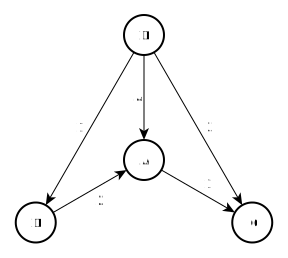
\includegraphics[width = \linewidth]{graphics/graph-eg-1.pdf}
          \caption{Nekonzistentan graf}
        \end{minipage}
        \hfill
        \begin{minipage}{0.45\linewidth}
          \centering
          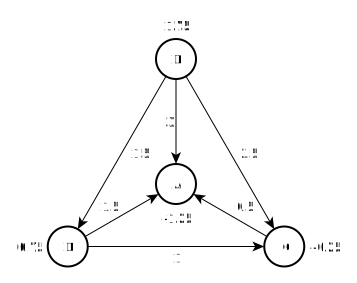
\includegraphics[width = 1.238\linewidth]{graphics/graph-eg-2.pdf}
          \caption{Konzistentan graf}
        \end{minipage}
      \end{figure}}
  \end{frame}

  \begin{frame}
    \frametitle{Metoda potencijala}
    \begin{itemize}
      \item ni \alert{graf toka preferencija} ne definira \emph{poredak} dobara
      \item \alert{metoda potencijala} definira \emph{poredak} dobara, i daje \alert{mjeru konzistentnosti} grafa
      \item \alert{mjera konzistentnosti} opisuje koliko je odluka donesena na temelju grafa \emph{pouzdana}
    \end{itemize}
  \end{frame}

  \section{Praktični dio}
  \begin{frame}
    \frametitle{Implementacija}
    \begin{itemize}
      \item \alert{\textit{Python}}
    \end{itemize}
  \end{frame}

  \begin{frame}
    \frametitle{Rezultati simulacije}
  \end{frame}

  \section{Zaključak}
  \begin{frame}
    \frametitle{Zaključak}
  \end{frame}

  \begin{frame}
    \frametitle{Hvala na pažnji!}
    \centering \Huge Pitanja?
\end{frame}
  
\end{document}